\subsubsection{Geometry and Dynamics}
\index{Kaimanovich, Vadim}

\paragraph{Research Team}
Vadim Kaimanovich (Professor), Michael Thon (PhD Student)

\medskip

The geometrical approach is currently becoming more and more popular
and useful, increasingly replacing more traditional analytic
considerations in various areas of mathematics and leading to
creation of new mathematical disciplines (geometric group theory,
non-commutative geometry etc.). Dynamics is inherently present in
this approach both in the form of the usual one-dimensional time
evolution (deterministic as well as stochastic) and in the form of
``non-commutative dynamics'' associated with various symmetries of
considered systems.

The subject area of what may be called ``Geometry and Dynamics''
intersects with numerous mathematical disciplines. More concretely,
my active research interests include the following topics:

\begin{itemize}

\item

Hyperbolic geometry

\item

Semi-simple Lie groups, their lattices and symmetric spaces

\item

Rigidity of groups and actions

\item

Geometric and combinatorial group theory

\item

Functional analysis on groups and groupoids, amenability

\item

C*-algebras and non-commutative geometry

\item

Spectral theory of groups, graphs and manifolds

\item

Foliations, laminations and equivalence relations

\item

Geometry of Teichm\"{u}ller and outer spaces

\item

Dynamics on groups and manifolds; geometric flows

\item

Geometrical aspects of conformal dynamics

\item

Probabilistic methods on algebraic and geometric structures

\item

Asymptotic theory of Markov chains

\item

Stochastic Loewner evolution and conformal field theory

\item

Theory of cocycles; cohomology of groups and varieties

\item

Ergodic theory

\end{itemize}



\paragraph{Highlights}

This year my research was mostly concentrated around understanding
singularity of harmonic measures arising from random walks on
hyperbolic spaces.

\begin{figure}[ht]
  \begin{center}
    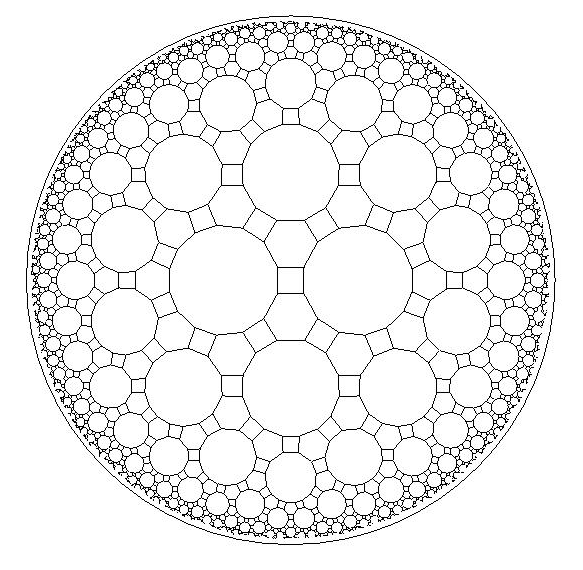
\includegraphics[width=\hsize]{Kaimanovich/profkaimanovich-fig1.png}
    \caption{ A typical Cayley graph of a hyperbolic group}\label{fig:profkaimanovich1}
   \end{center}
\end{figure}

The question whether the harmonic measure has maximal dimension has
a long history in various areas (classical harmonic analysis,
conformal dynamics, periodic negatively curved manifolds, continuous
fractions). It is notoriously difficult, but all known answers
indicate that the maximal dimension of the harmonic measure should
imply that the considered system is distinguished by much higher
symmetries within a given class.

One can conjecture that a finitely supported random walk on a
hyperbolic group may have maximal entropy if and only if the group
is a finite extension of a free group. Note that if one is allowed
to consider not necessarily finitely supported measures, then recent
results show existence of maximal entropy random walks on an
arbitrary hyperbolic group.

The ``difficult'' part of the above conjecture is showing that
existence of a maximal entropy random walk implies that the group is
a finite extension of a free group. However, in spite of a complete
structure theory for finite extensions of free groups, we still do
not know whether any such group carries a finitely supported maximal
entropy random walk.

\begin{figure}[ht]
  \begin{center}
    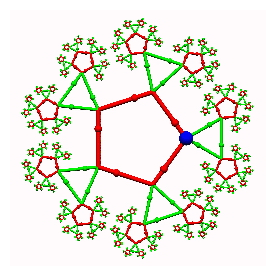
\includegraphics[width=\hsize]{Kaimanovich/profkaimanovich-fig2.png}
    \caption{ The free product of cyclic groups of orders 3 and 5}\label{fig:profkaimanovich2}
   \end{center}
\end{figure}

We look at the particular case when the group is the free product of
finitely many finite groups. The main result is that, generically,
in this situation no random walk has maximal entropy. The proof is
based on the fact that the harmonic measure in this situation is
\emph{multiplicative Markov} (Mairesse and Matheus). Since Patterson
$(\equiv$ maximal entropy) measure on the boundary is also
multiplicative Markov, the standard symbolic dynamics tools
(uniqueness of the maximal entropy measure for topological Markov
chains) become much easier to apply.


\paragraph{Organization}
% list the (research) events you have organized, if any,


\begin{enumerate}
\item  Organizer of the Spring School in Probability at the Schr\"{o}dinger
Institute (ESI), Vienna, Austria, 2006.

\item  Organizer of the special semester \textit{Amenability} at the
Schr\"{o}dinger Institute (ESI), Vienna, Austria, 2007.

\end{enumerate}

\paragraph{Collaborations}

\begin{enumerate}
\item {\sl State Univeristy of New York at Stony Brook, USA, University of
Toronto, Canada} \\
Prof.~M. Lyubich \\
Measures in conformal dynamics

\item {\sl Univeristy of Illinois at Urbana-Champaign, USA} \\ Prof. Ilya Kapovich,
Prof.~P. Schupp\\
Metric properties of free group automorphisms

\item {\sl Texas A\& M University, USA} \\
Prof.~R. Grigorchuk, Prof.~V. Nekrashevych\\
Ergodic methods in group theory

\item {\sl Universit\'e de Gen\`eve, Switzerland} \\
Prof.~T Nagnibeda \\
Ergodic properties of boundary actions

\item {\sl ETH Z\"urich, Switzerland}\\
Prof.~M. Burger, graduate student T. B\"uhler \\
Amenability of groupoids

\item {\sl Schr\"{o}dinger Institute, Vienna, Austria}\\
Prof.~K. Schmidt \\
Ergodic properties of cocycles

\item{\sl Universit\'e de Vannes, France}\\
Dr.~V. Le Prince \\
Singularity of the harmonic measure

\item{\sl University of Lisbon, Portugal}\\
Dr.~P. Freitas \\
Compactifications of symmetric spaces

\item{\sl Universit\'e Paris-7, France}\\
Dr.~J. Mairesse \\
Queuing systems and harmonic measures
\end{enumerate}



\paragraph{Grants}
\begin{enumerate}
\item Funded by European Union, Marie Curie Research Training
Network FP6, \emph{Conformal structures and dynamics' (CODY)},
network of 10 European countries, member of the German node.
\end{enumerate}

\nocite{Kaimanovich1}\nocite{Kaimanovich2} \nocite{Kaimanovich3}
